\documentclass[18pt, a0paper, portrait]{tikzposter}
\usepackage[magyar]{babel}
\usepackage[utf8]{inputenc}
\usepackage{float}
\usepackage[T1]{fontenc}
\usepackage{amsmath}
\usepackage{graphicx}
\graphicspath{{/home/istvan/insar/images/}}
\usepackage{siunitx}
\usepackage{subfig}
\usepackage{caption}
\DeclareGraphicsExtensions{.png,.jpg,.jpeg}

\title{\parbox{\linewidth}{\centering Felszíni deformációk meghatározása a
Csomád vulkán térségében archív Envisat felvételek alapján}}
\author{Bozsó István, Szűcs Eszter, Bányai László, Wesztergom Viktor}
\institute{MTA CSFK Geodéziai és Geofizikai Intézet}
\date{2017.04.07}

\makeatletter
\newcommand\insertlogoi[2][]{\def\@insertlogoi{\includegraphics[#1]{#2}}}
\newcommand\insertlogoii[2][]{\def\@insertlogoii{\includegraphics[#1]{#2}}}
\newlength\LogoSep
\setlength\LogoSep{0pt}

\insertlogoi[width=6.5cm]{ggi_logo.png}
\insertlogoii[width=6.5cm]{esa_logo.eps}

\renewcommand\maketitle[1][]{  % #1 keys
    \normalsize
    \setkeys{title}{#1}
    % Title dummy to get title height
    \node[transparent,inner sep=\TP@titleinnersep, line width=\TP@titlelinewidth, anchor=north, minimum width=\TP@visibletextwidth-2\TP@titleinnersep]
        (TP@title) at ($(0, 0.5\textheight-\TP@titletotopverticalspace)$) {\parbox{\TP@titlewidth-2\TP@titleinnersep}{\TP@maketitle}};
    \draw let \p1 = ($(TP@title.north)-(TP@title.south)$) in node {
        \setlength{\TP@titleheight}{\y1}
        \setlength{\titleheight}{\y1}
        \global\TP@titleheight=\TP@titleheight
        \global\titleheight=\titleheight
    };

    % Compute title position
    \setlength{\titleposleft}{-0.5\titlewidth}
    \setlength{\titleposright}{\titleposleft+\titlewidth}
    \setlength{\titlepostop}{0.5\textheight-\TP@titletotopverticalspace}
    \setlength{\titleposbottom}{\titlepostop-\titleheight}

    % Title style (background)
    \TP@titlestyle

    % Title node
    \node[inner sep=\TP@titleinnersep, line width=\TP@titlelinewidth, anchor=north, minimum width=\TP@visibletextwidth-2\TP@titleinnersep]
        at (0,0.5\textheight-\TP@titletotopverticalspace)
        (title)
        {\parbox{\TP@titlewidth-2\TP@titleinnersep}{\TP@maketitle}};

    \node[inner sep=0pt,anchor=west]
      at ([xshift=-\LogoSep]title.west)
      {\@insertlogoi};

    \node[inner sep=0pt,anchor=east]
      at ([xshift=\LogoSep]title.east)
      {\@insertlogoii};

    % Settings for blocks
    \normalsize
    \setlength{\TP@blocktop}{\titleposbottom-\TP@titletoblockverticalspace}
}

\renewenvironment{tikzfigure}[1][]{
  \def \rememberparameter{#1}
  \vspace{10pt}
  \refstepcounter{figurecounter}
  \begin{center}
  }{
    \ifx\rememberparameter\@empty
    \else %nothing
    \\[10pt]
    %{\small Fig.~\thefigurecounter: \rememberparameter}
    {\small \rememberparameter}
    \fi
  \end{center}
}

\makeatother

\usetheme{Autum}

\tikzposterlatexaffectionproofoff

\begin{document}

\maketitle

\block[]{Bevezetés}
{
    Az európai kontinentális litoszféra szeizmikus szempontból aktív zónája az,
    ún. Kárpát-kanyar, ahol gyakoriak a lemezen belüli (intraplate) közepes
    mélységű (sub-crustal) földrengések, melyeket jelentős energia
    felszabadulása kísér. Ebben a zónában található a Kárpát-Pannon térség
    legfiatalabb vulkánja a Csomád. A vulkán térségében, elvégzett geofizikai
    és geológiai vizsgálatok kimutatták, hogy a vulkán egy potenciálisan aktív
    magmakamrát rejt magában. A felszíni deformációk becslése segítheti a
    múltbéli és jelenkori geodinamika megértését és a folyamatok feltérképezését.
    Az ESA CAT-1 pályázat keretében szerzett SAR műholdfelvételekből (Envisat, 2002-2010)
    képzett interferogramok felhasználásával végzett idősorelemzéssel meghatározhatóak
    a műhold irányú (LOS) átlagos sebességek mind felszálló (ASC) mind leszálló
    (DES) irány esetén. Az intézetben kifejlesztett DAISY program segítségével
    az ASC és DES irányú sebességek vertikális és kelet-nyugati komponense
    meghatározható. Az alábbiakban bemutatjuk a feldolgozás során elért eredményeket
    és összehasonlítjuk azokat a korábbi GNSS mérések eredményeivel, továbbá
    ismertetjük az InSAR módszer korlátait.
}

\begin{columns}
    \column{0.5}
    \block[]{DInSAR alapelv}
    {
        \begin{center}
            \begin{minipage}{0.45\linewidth}
                \centering
                \begin{tikzfigure}[DInSAR alapelv. Felszíni deformáció a két
                kép készítése között eltelt időpontban fáziskülönbséget
                eredményez. Gareth Funning tulajdona.]
                    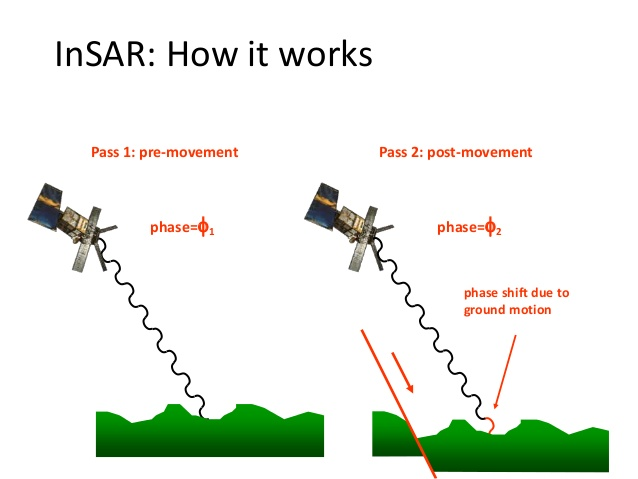
\includegraphics[height=15cm]{DInSAR_concept.jpg}
                \end{tikzfigure}
            \end{minipage}\hfill
            \begin{minipage}{0.45\linewidth}
                \centering
                \begin{tikzfigure}[2014-es kumamoto-i földrengés előtt és után
                                   készített SAR képből előállított interferogram]
                    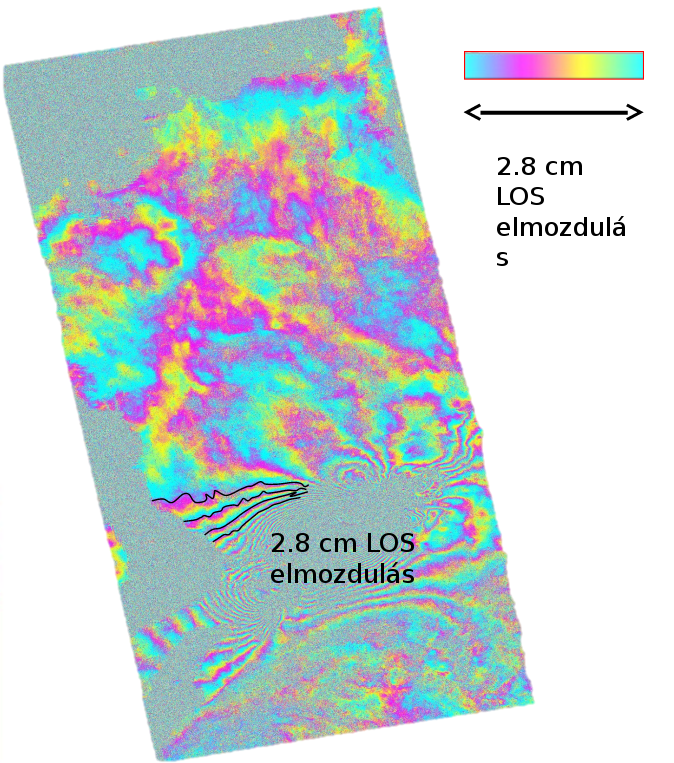
\includegraphics[width=0.75\linewidth]{earthquake_ifg.png}
                \end{tikzfigure}
            \end{minipage}
        \end{center}
        \vspace{0.75cm}

        \begin{itemize}
            \item SAR - mikrohullámú radar technika: $\lambda =
            \SI{5.6}{\centi\meter}$
            \item két felvétel közötti fáziskülönbség $\rightarrow$
            deformációra lehet következtetni
            \item csak műhold látóirányú (line-of-sight, LOS) deformáció
            észlelhető
            \item limitáló tényező: atmoszféra állapotának megváltozása két
            felvétel között, felvételek nagy térbeli és időbeli szeparáltsága
            (nagy térbeli és időbeli bázisvonalak)
            \item nehézség: $ 2 \pi$ fáziskülönbség a két felvétel eltelte között
        \end{itemize}
    }

    \block[]{InSAR idősor elemzés archív ESA Envisat felvételek alapján}
    {
        \begin{itemize}
            \item lassú tektonikus folyamatok megfigyelése $\rightarrow$ kis
            időbeli és térbeli bázisvonalú interferogram sorozattal
            \item nagy időbeli és térbeli bázisvonalak $\rightarrow$ felszín
            reflexiós tulajdonsága megváltozik $\rightarrow$ koherencia
            elvesztése
            \item PSI bázisvonalak esetében a koherencia sok interferogram
            esetén elveszik
            \item \textbf{megoldás:} interferogramok fáziskülönbségeiből 1D-s
            hálózat létrehozása $\rightarrow$ invertálás $\rightarrow$
            deformációk; koherens interferogramok megtartása; SBAS hálózat
            felépítése a lehető legtöbb redundanciával (ellenőrzés)
        \end{itemize}

        \begin{center}
            \begin{minipage}[t]{0.45\linewidth}
                \centering
                \begin{tikzfigure}[Példa zajos interferogramra, a
                fázisváltozás a két felvétel, 2003.09.13.-2004.03.06. ($\Delta
                T= 175$ nap, $B_{\perp} = \SI{61}{\meter}$) között
                véletlenszerű. Némi koherencia tapasztalható a városi
                környezetben.]
                    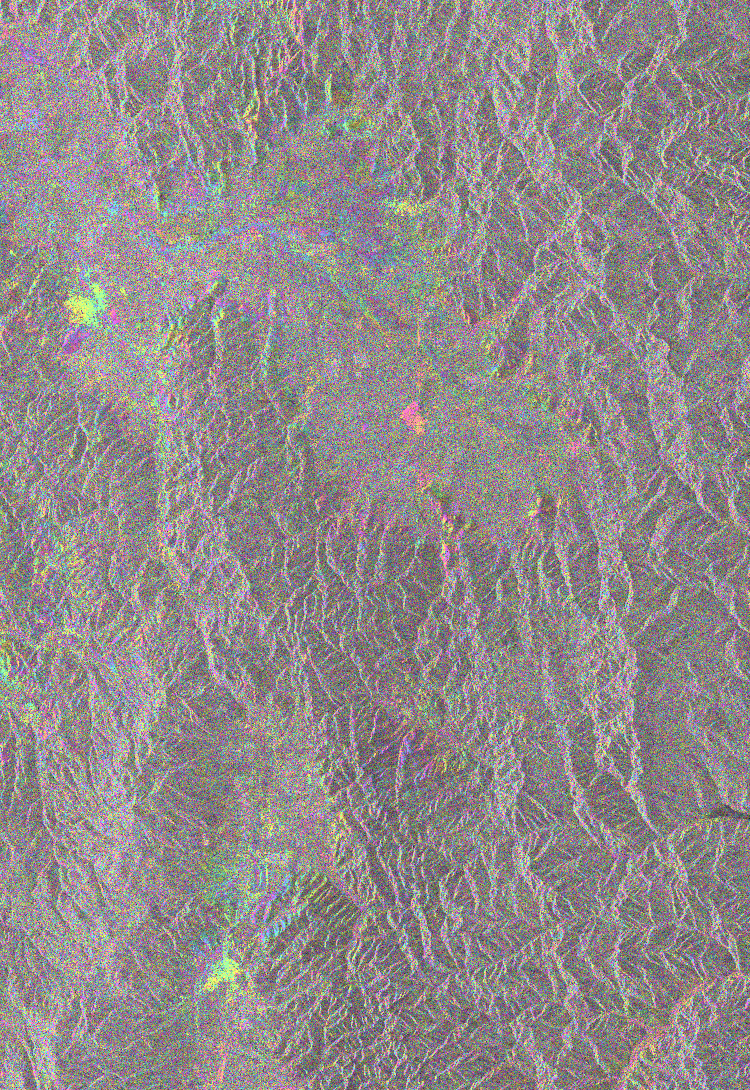
\includegraphics[height=10cm]{ifg_bad.png}
                \end{tikzfigure}
            \end{minipage}\hfill
            \begin{minipage}[t]{0.45\linewidth}
                \centering
                \begin{tikzfigure}[Példa koherens interferogramra, a felvétel
                időpontjai: 2003.09.13.-2004.03.06. ($\Delta T= 70$ nap,
                $B_{\perp} = \SI{95}{\meter}$). Az interferogram döntően
                atmoszferikus hatást tükröz.]
                    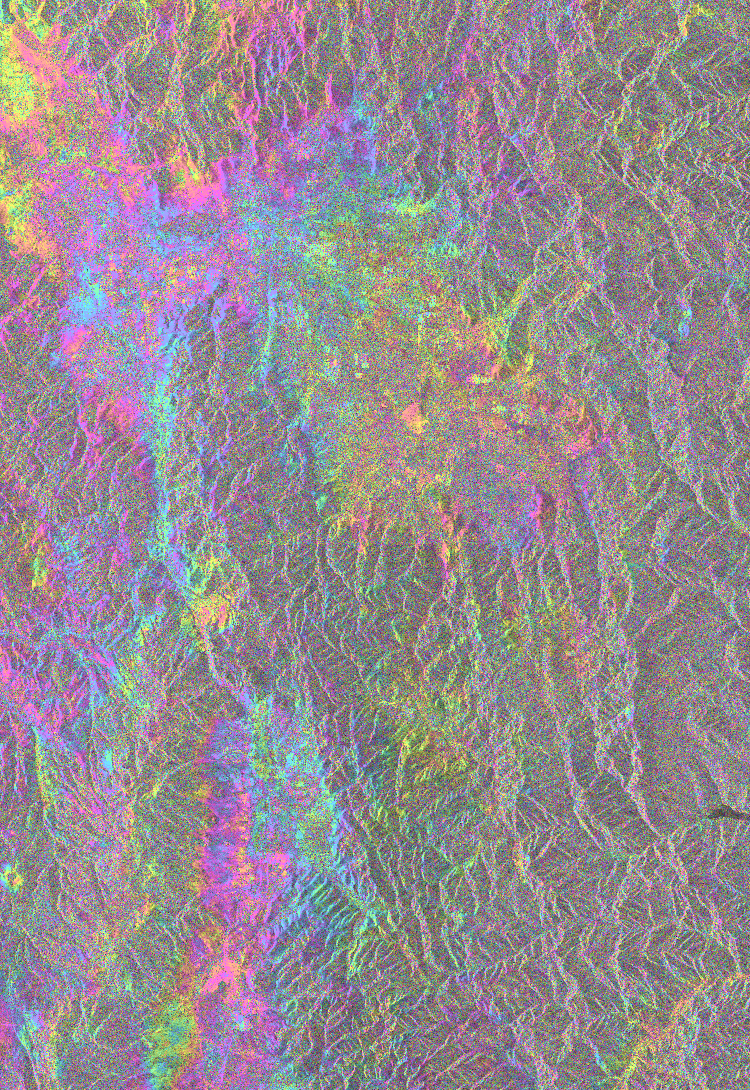
\includegraphics[height=10cm]{ifg_good.png}
                \end{tikzfigure}
            \end{minipage}
        \end{center}
        \vspace{0.75cm}

        \begin{center}
            \begin{minipage}[t]{0.45\linewidth}
                \centering
                \begin{tikzfigure}[Felszálló irányú SBAS hálózat]
                    \includegraphics[width=0.7\linewidth]{asc_sb.png}
                \end{tikzfigure}
            \end{minipage}
            \begin{minipage}[t]{0.45\linewidth}
                \centering
                \begin{tikzfigure}[Leszálló irányú SBAS hálózat]
                    \includegraphics[width=0.7\linewidth]{des_sb.png}
                \end{tikzfigure}
            \end{minipage}
        \end{center}

    }


    \column{0.5}
    \block[]{Egy interferogram pixel fázisának tagjai}
    {
        \[
            \Delta\Phi = \Phi_{\text{def}} + \Delta\Phi_{\text{DEM}} +
            \Delta\Phi_{\text{atmo}} + \Delta\Phi_{\text{orb}} +
            \Phi_{\text{zaj}}
        \]

        \begin{itemize}
            \item $\Phi_{\text{def}}$ - a deformációs jel
            \item $\Delta\Phi_{\text{DEM}}$ - digitális magassági modell
            hibájából származó fázis
            \item $\Delta\Phi_{\text{atmo}}$ - atmoszferikus jel
            \item $\Delta\Phi_{\text{orb}}$ - műholdpálya hiba
            \item $\Phi_{\text{zaj}}$ - egyéb hiba- és zajtényezők
        \end{itemize}

        \textbf{Feladat}: a $\Phi_{\text{def}}$ becslése és a fázis
        kicsomagolása (unwrapping: a [0, 2pi) tartományon adott fázis értékek
        integrálása a relatív deformációk meghatározására)
    }

    \block[]{Eredmények és összevetésük korábbi GPS adatokkal, összefoglalás}
    {
        \begin{minipage}[t]{0.5\linewidth}
            \begin{tikzfigure}[GPS mérésekből számított (Hoeven et al. 2005,
            \cite{Hoeven:2005}) és InSAR vertikális sebességkomponensek
            összehasonlítása. A két sebességmező hasonló térbeli eloszlást
            mutat, de felfedezhetőek eltérések.]
                \includegraphics[height=18.7cm]{gps_vs_insar_vert.png}
            \end{tikzfigure}
        \end{minipage}
        \begin{minipage}[t]{0.5\linewidth}
            \begin{center}
            \begin{tikzfigure}[1997 és 2004 között végzett GPS mérések alapján
            számított vertikális sebességek (Hoeven et al. 2005,
            \cite{Hoeven:2005}). A kihelyezett GPS állomások pontjaiban nyilak
            mutatják a vertikális sebességkomponensek értékeit. A
            hibaellipszisek a 95\%-os konfidencia intervallumot mutatják. Az
            interpolált sebességék értékei a színskála segítségével
            olvashatóak le az ábráról.]
                \includegraphics[height=14.8cm]{hoeven_gps_with_graticule.png}
            \end{tikzfigure}
            \end{center}
        \end{minipage}
        \vspace{0.25cm}

        \innerblock{Összefoglalás}
        {
            A Vrancea-beli geodinamikai folyamatok vizsgálatára korábban több
            GNSS mérési kampányt is folytattak (Hoeven et al. 2005,
            \cite{Hoeven:2005}; Schmitt et al. 2007, \cite{Schmitt:2007}).
            Ezek bizonyos területeken ellentmondó eredményeket adtak. A
            műholdradar interferometria egy független ellenőrzési lehetőséget
            ad a felszíni deformációk meghatározására. A Csomád vulkánt
            közrefogó terület a GNSS méréseknél a TUSN és a ZABA pontok között
            helyezkednek el.  A StaMPS és DAISY programokból származó
            négyzetrácsra interpolált vertikális sebességek, mind irányukban,
            mint magnitúdójukban jó relatív egyezést mutatnak a le- és
            felszálló Envisat felvételekből meghatározott sebesség értékekkel,
            annak ellenére is, hogy viszonylag kedvezőtlen a felvételi
            geometria. A 2014-ben pályára bocsájtott ESA Sentinel-1 műholdpár
            esetén a teljes földfelszín szisztematikus  (6 naponkénti)
            leképezése valósul meg, mely jelentősen javítani fogja a kis
            elmozdulásokkal járó deformációk térképezését.
        }

        \vspace{-0.75cm}

        \begin{thebibliography}{2}
            \bibitem{Hoeven:2005}
            A.G.A. van der Hoeven, V. Mocanu, W. Spakman, M. Nutto, A.
            Nuckelt, L. Matenco, L. Munteanu, C. Marcu, B.A.C. Ambrosius:\\
            Observation of present-day tectonic motions in the Southeastern
            Carpathians: Results of the ISES/CRC-461 GPS measurements\\
            Earth and Planetary Science Letters 239 (2005) 177--184,
            doi:10.1016/j.epsl.2005.09.018

            \bibitem{Schmitt:2007}
            Günter Schmitt, Andre Nuckelt, Andreas Knöpfler, Constantin
            Marcu:\\
            Three dimensional plate kinematics in Romania\\
            International Symposium on Strong Vrancea Earthquakes and Risk
            Mitigation Oct. 4--6, 2007, Bucharest, Romania

        \end{thebibliography}
    }

\end{columns}

\end{document}
